\documentclass[9pt]{beamer}
%\usepackage{amsmath,amssymb,amsthm,tikz-cd}
\usetheme{Madrid}
\usecolortheme{default}
\DeclareMathOperator{\Hom}{Hom}
\DeclareMathOperator{\Det}{det}
\DeclareMathOperator{\supp}{supp}

\title[Differentiable manifolds and the Hairy Ball Theorem]
{Differentiable manifolds and the Hairy Ball Theorem}

\author[Jonathan Lau] % (optional)
{Jonathan Lau}

\AtBeginSection[]
{
	\begin{frame}
		\frametitle{Table of Contents}
		\tableofcontents[currentsection]
	\end{frame}
}

\begin{document}
	
\frame{\titlepage}

\begin{frame}
	\frametitle{Table of Contents}
	\tableofcontents
\end{frame}

\section{Manifolds}
	
\begin{frame}
    \begin{block}{Charts}
        A chart on a topological space $M$ is a pair $(U, \phi)$ where $U\subset M$ and $\phi:U\rightarrow \mathbb{R}^n$ is a homeomorphism.
    \end{block}

    Sometimes, we express $\phi$ as $(x_1, \dots, x_n)$.

    \begin{block}{Manifolds}
        A $n$ dimensional manifold $M$ is a subset of $\mathbb{R}^\ell$ together with a collection of charts $\mathcal{A}$ that cover $M$ such that for all charts $(U, \phi)$, $(V, \psi)$, the maps $\psi\circ\phi^{-1}$ and $\phi\circ\psi^{-1}$ are smooth on $\phi(U\cap V)$ and $\psi(U\cap V)$ respectively.
    \end{block}
    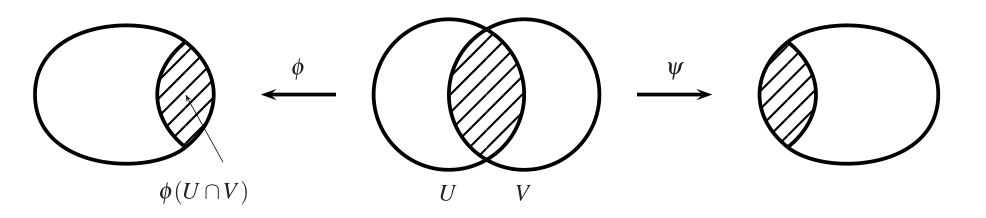
\includegraphics[scale=0.6]{compatible.PNG}
\end{frame}

\begin{frame}
    \begin{block}{Tangent Space}
        Given a point $p\in M$ and a smooth curve $\gamma:(-1,1)\rightarrow M$ in $M$ such that $\gamma(0)=p$, its velocity vector is $\frac{d\gamma}{dt}\vert_{t=0}$. The set of all velocity vectors at $p$ is the tangent space at $p$, denoted $T_p M$.
    \end{block}
    With a chart $(U, \phi)$ such that $\phi(p)=0$, construct curves $\gamma_i:t\mapsto \phi^{-1}\circ\iota_i(t)$, where $\iota_i$ is the inclusion into the $i$th coordinate. Their velocity vectors form a basis for the tangent space.

    Example: sphere
\end{frame}

\begin{frame}
    \begin{block}{Smooth Functions}
        A continuous function $F:N\rightarrow M$ is smooth if for all charts $(U, \phi)$ on $N$ and $(V, \psi)$ on $M$, $\psi\circ F\circ \phi^{-1}$ is smooth.
    \end{block}
    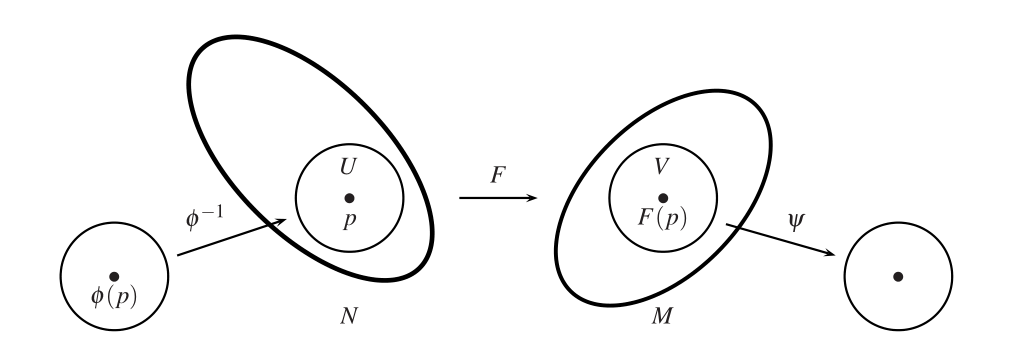
\includegraphics[scale=0.55]{smooth_function.PNG}
\end{frame}

\begin{frame}
    \begin{block}{1-form}
        A 1-form $\omega$ is a linear function from $T_p M$ to $\mathbb{R}$.
    \end{block}
    The space of 1-forms $\Hom(T_p M, \mathbb{R})$ is a vector space of dimension $n$. If we fix a basis for $T_pM$, then we can express vectors in $T_pM$ in terms of the coordinates in that basis. Then, we define $dx_i(a_1, \dots, a_n) = a_i$.
    \begin{block}{$k$-form}
        A $k$-form $\omega$ is an alternating multilinear function from $(T_p M)^k$ to $\mathbb{R}$.
    \end{block}
\end{frame}

\begin{frame}
    \begin{block}{Theorem}
        $\{dx_{i_1}\wedge\dots\wedge dx_{i_k}|1\leq i_i<\dots<i_k\leq n\}$ is a basis for $\Lambda^k(T_pM)$, the set of alternating multilinear functions on $(T_pM)^k$.
    \end{block}
    This theorem shows that $dx_1, \dots, dx_n$ is a basis for the vector space of 1-forms. With this basis, we can express all 1-forms $\omega$ as $(a_1, \dots, a_n)$. For a vector $v=(b_1, \dots, b_n)\in T_pM$, \begin{align*}\omega(v)=&(a_1dx_1+\dots+a_ndx_n)(b_1,\dots,b_n)\\
        =&a_1dx_1(b_1, \dots, b_n)+\dots+a_ndx_n(b_1, \dots, b_n)\\
        =&a_1b_1+\dots+a_nb_n
    \end{align*}
    So, a 1-form $\omega$ maps tangent vectors to the length of their projection onto the subspace spanned by $\omega$, up to a multiplicative constant $|\omega|$.
\end{frame}

\begin{frame}
    \begin{block}{Wedge Product}
        The wedge product of $k$ 1-forms $\omega_1, \dots, \omega_k$ is the k-form $\omega_1\wedge\dots\wedge\omega_k(v_1, \dots, v_k)=\Det(\omega_i(v_j))$.
    \end{block}
    Consider a 3-form $dx_1\wedge dx_2\wedge dx_3$ on $T_p\mathbb{R}^5$, and apply it to the vectors $u=(0,0,1,1,1), v=(1,2,0,0,1), w=(2,2,2,1,0)$. The result is $\Det\begin{pmatrix} 0 & 1 & 2 \\
        0 & 2 & 2 \\
        1 & 0 & 2
    \end{pmatrix}$. This is the same as projecting $u,v,w$ onto the subspace ${(c_1,c_2,c_3,0,0)}$, then calculating it's volume.

    By the Gram Schmidt process, $\omega_1\wedge\dots\wedge\omega_k=c\tau_1\wedge \dots\wedge\tau_k$ where $\tau_1,\dots,\tau_k$ are orthonormal. Then, \begin{align*}\omega_1\wedge\dots\wedge\omega_k(v_1,\dots,v_k)=&c\tau_1\wedge \dots\wedge\tau_k(v_1,\dots,v_k)\\=&c\Det(\tau_i(v_j)),\end{align*} which is projecting the $v_i's$ onto the subspace spanned by the $\tau_i's$, then taking the hypervolume and multiplying by a constant $c$.
    

\end{frame}

\begin{frame}
    \begin{block}{Differential Forms}
        A differential form $\omega$ is an object where at each $p\in M$, $\omega_p$ is a $n$-form on $T_pM$, and for all charts $(U, x_1, \dots, x_n)$, $\omega=f(p)dx_1\wedge\dots\wedge dx_n$ for some smooth $f$.
    \end{block}

    Example: $dx_1$ is a differential 1-form.

    \begin{block}{The $d$ operator}
        Let $f:M\rightarrow \mathbb{R}$ be a smooth function. We define a differential 1-form $df$ as $\sum_{i=1}^n \frac{\partial f}{\partial x_i}dx_i$.
        Given a differential form $\omega$ on $M$ and a chart $(U, \phi)$, $\omega=\sum_I f dx_I$ on $U$. Then, on $U$, $d\omega$ is defined as $\sum_I df\wedge dx_I$.
    \end{block}

\end{frame}

\section{Integration of Differential $n$-Forms}
\begin{frame}
    \begin{block}{Orientation}
        stuff ...
    \end{block}
\end{frame}

\begin{frame}
    \begin{block}{Manifolds with Boundary}
        stuff ...
    \end{block}
\end{frame}

\begin{frame}
    \begin{block}{Integration on a $\mathbb{R}^n$}
        Let $\omega$ be a $n$-form on $(U, \phi)$, where $U\subset\mathbb{R}^n$. Then $\omega=f(x)dx_1\wedge\dots\wedge dx_n$ for some smooth $f$. The integral of $\omega$ over $U$, denoted $\int_U\omega$, is defined to be $\int_U f$.
    \end{block}

    \begin{block}{Pullback}
        ...
    \end{block}

    \begin{block}{Integration on a chart}
        Let $\omega$ be a $n$-form on $U$. The integral of $\omega$ over $U$ is defined as 
    \end{block}
\end{frame}

\begin{frame}
    \begin{block}{Partition of Unity}
        A partition of Unity on a manifold $M$ is a collection of nonnegative smooth functions $\{\rho_\alpha:M \rightarrow \mathbb{R}\}_{\alpha\in A}$ such that \begin{enumerate}[i]
            \item the collection of supports, $\{\supp\rho_\alpha\}_{\alpha\in A}$, is locally finite,
            \item $\sum_{\alpha\in A} \rho_\alpha = 1.$
        \end{enumerate}
    \end{block}

    \begin{block}{Integration on a Manifold}
        Let $\omega$ be a $n$-form on $M$. The integral of $\omega$ over $M$, denoted by $\int_M \omega$, is defined to be $\sum_{\alpha\in A}\int_{U_\alpha}\rho_\alpha\omega$.
    \end{block}
\end{frame}

\begin{frame}
    \begin{block}{Stokes' theorem on $\mathcal{H}^n$}
        stuff ...
    \end{block}
\end{frame}

\begin{frame}
    \begin{block}{Stokes' theorem on Manifolds}
        stuff ...
    \end{block}
\end{frame}

\section{The Hairy Ball Theorem}

\begin{frame}
    \begin{block}{stuff}
        stuff ...
    \end{block}
\end{frame}

\end{document}